% -----------------------------------------------------------------------------------
% MammAlps Pipeline Update – 10–15 min Beamer presentation
% (compile with xelatex)
% -----------------------------------------------------------------------------------

% Changelog (2025‑06‑10, pass 3)
%   • Figures now reference the exact paths from the original paper
%   • Removed placeholder graphics that were not in the source repo
% -----------------------------------------------------------------------------------

\documentclass[aspectratio=169,xcolor=dvipsnames,t]{beamer}

% ---- PACKAGES & THEME ----
\usepackage{fontspec}
\usetheme{SimplePlusAIC}
\usepackage{hyperref}
\usepackage{graphicx}
\usepackage{booktabs}
\usepackage{svg}
\usepackage{tikz}
\usepackage{makecell}
\usepackage{wrapfig}

% ---- TITLEPAGE INFO ----
\title[MATH-454]{Parallelizing SWE simulations with MPI and CUDA}
\subtitle{MATH-454 Final Project}
\author[Aaron Dinesh]{Aaron Dinesh}
\institute[EPFL]{EPFL}
\date{\today}

% ----------------------------------------------------------------
\begin{document}
% ----------------------------------------------------------------
\maketitlepage

% ----------------------------------------------------------------
\begin{frame}[t]{Overview}
  \tableofcontents[hideallsubsections]
\end{frame}

\makesection{MPI Parallelism}

\begin{frame}{Domain Decomposition}{Tkiz Overlay}
  \begin{columns}[c]            % [c] = vertical-center all columns
    % ---------- LEFT TEXT ----------
    \begin{column}{0.55\linewidth}
      \Large                 % any text you like here
      \textbf{Halo exchange} splits the domain
      into overlapping blocks so that each MPI
      task can update ghost cells locally
    \end{column}

    % ---------- RIGHT IMAGE ----------
    \begin{column}{0.45\linewidth}
      \centering
      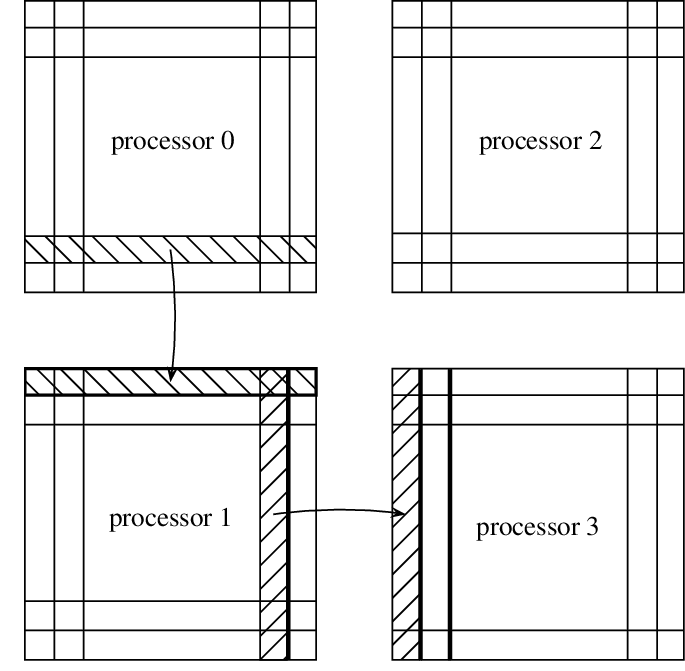
\includegraphics[width=\linewidth]{figs/HaloExchange.png}
      % or [width=.9\linewidth] if you want margins
    \end{column}
  \end{columns}
\end{frame}

\begin{frame}{Theoretical Scaling}
  \begin{columns}[c]
    \begin{column}{0.35\linewidth}
      \begin{itemize}
      \item \textbf{Amdahl's Law:} $T_p = \left[(1-\alpha) + \frac{\alpha}{p}\right]T_{1}$
      \item \textbf{Gustafson's Law:} $S(N, p) = 1 + (p-1)\alpha(N)$
      \end{itemize}
    \end{column}
    \begin{column}{0.65\linewidth}
      \centering
      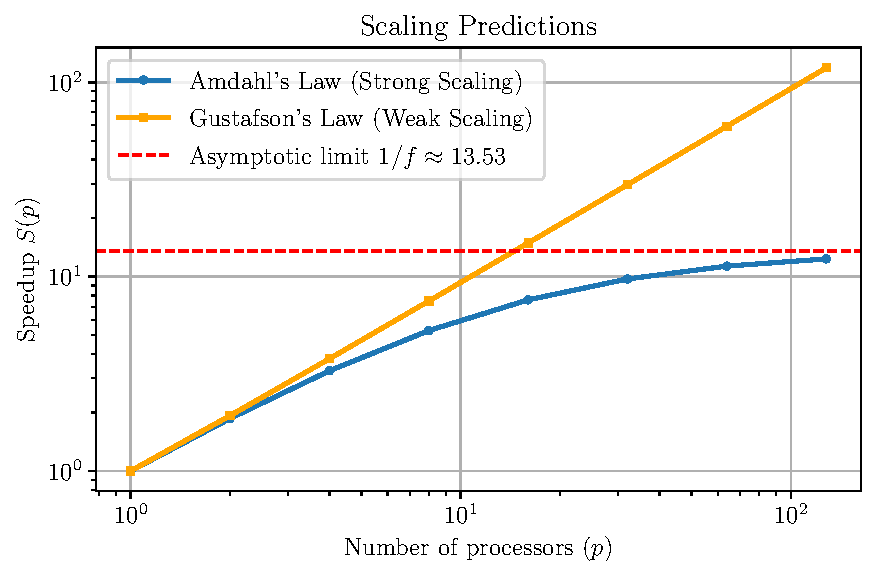
\includegraphics[width=\linewidth]{figs/scaling_laws.pdf}
    \end{column}
  \end{columns}
\end{frame}

% ----------------------------------------------------------------
\subsection{Parsing raw videos}
\begin{frame}{Step 1 — Raw video parser}
  \begin{itemize}
    \item Recurses through arbitrary directory trees (handles \texttt{DCIM/}, \texttt{BCF/} …).
    \item Groups clips into events when inactivity $>\,$\texttt{event\_time\_period\_s} (default 300 s).
    \item Writes tidy filenames and a single CSV with \emph{site}, \emph{camera}, \emph{event}, metadata.
  \end{itemize}
  \begin{block}{2024 improvement}
    Command‑line flag for gap length, more robust to different structures.
  \end{block}
\end{frame}

% ----------------------------------------------------------------
\subsection{MegaDetector V6}
\begin{frame}{Step 2 — MegaDetector V6 upgrade}
  \begin{itemize}
    \item Switched to \textbf{PyTorch‑Wildlife} implementation (YOLOv9/v10 backbone).
    \item Script rewritten: new I/O, batch API, GPU batching.
    \item Converted V6 JSON back to legacy V5 schema $\rightarrow$ zero downstream code changes.
  \end{itemize}
\end{frame}

% ----------------------------------------------------------------
\subsection{Trimming and tracking}
\begin{frame}{Steps 3 \& 4 — Trim $\rightarrow$ ByteTrack}
  \begin{itemize}
    \item \textbf{Trim} videos to animal spans ($\ge$30 frames, MD confidence $\ge$0.5).
    \item Reduces 56 h $\Rightarrow$ 11.1 h (80 \%).
    \item Run MD on every frame, then ByteTrack: Kalman + IoU association at 30 fps.
    \item Fixed frame‑index bug $\mapsto$ stable tracks, optional interpolation \& smoothing.
  \end{itemize}
\end{frame}

% ----------------------------------------------------------------
\subsection{Visual QA}
\begin{frame}{Step 5 — Visualising tracks}
  \begin{itemize}
    \item Auto‑renders annotated MP4s for batch QA.
    \item Produces an Excel‑ready CSV to flag \emph{false positives}, \emph{ID switches}, etc.
    \item Screenshot example ↓
  \end{itemize}
  \centering
  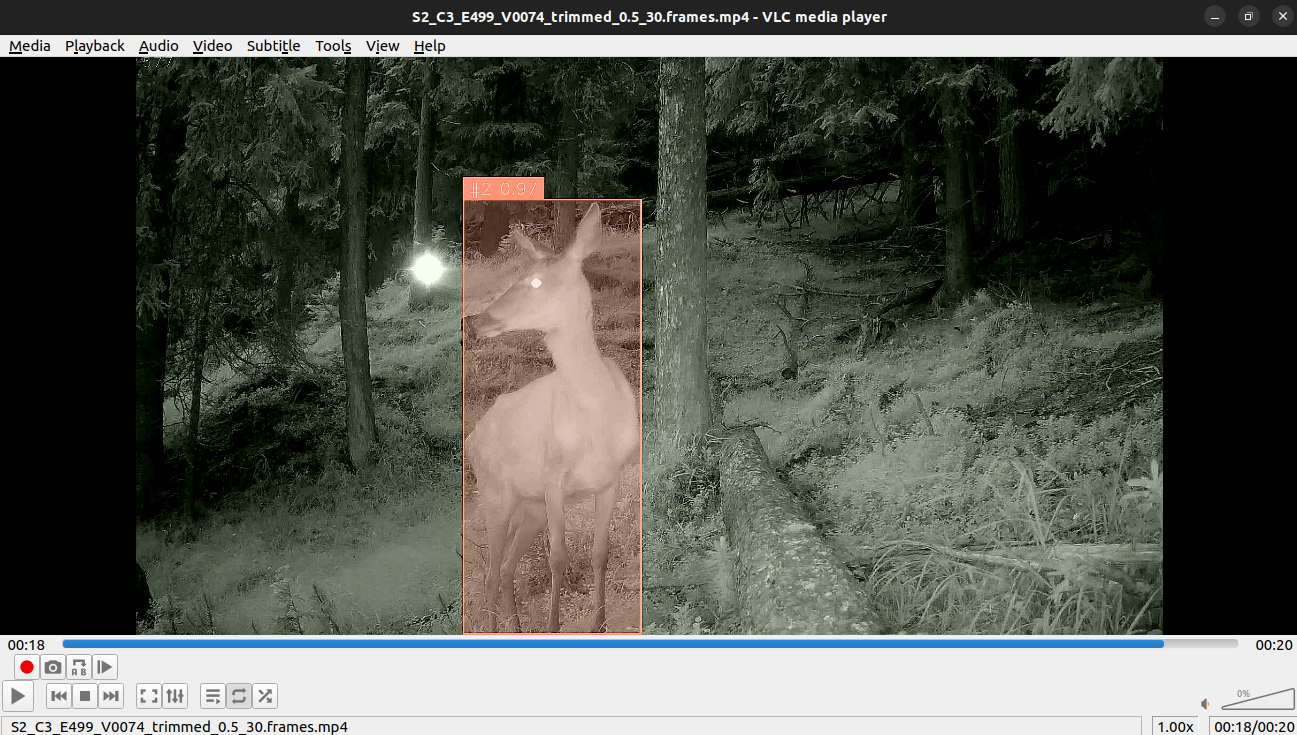
\includegraphics[width=.7\linewidth]{figs/vid.png}
\end{frame}

% =================================================================
% SECTION: 2024 dataset insights
% =================================================================
\makesection{2024 Data — Key Numbers}

\begin{frame}{Field campaign 2024}
  \begin{itemize}
    \item 9 Bushnell cameras, 3 sites (alpine meadow, forest edge, scree field).
    \item 56 h raw footage (June–August 2024, day \& IR night).
    \item \textbf{1,050 events} detected across sites.
  \end{itemize}
\end{frame}

\begin{frame}{Event distribution}
  \begin{columns}[T]
    \begin{column}{0.55\linewidth}
      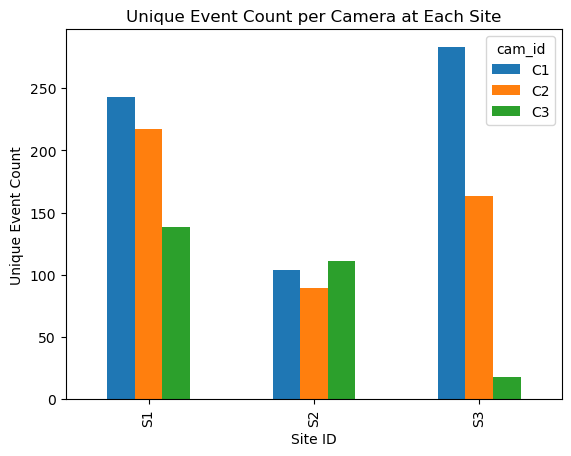
\includegraphics[width=\linewidth]{figs/raw/event_count_per_camera.png}
    \end{column}
    \begin{column}{0.45\linewidth}
      \small
      \begin{itemize}
        \item Site 1 \& 3 dominate — $\sim$400 events each.
        \item Site 3/C3 malfunction $\rightarrow$ only 15 events.
      \end{itemize}
    \end{column}
  \end{columns}
\end{frame}

\begin{frame}{Animal presence \& trimming impact}
  \begin{columns}[T]
    \begin{column}{0.48\linewidth}
      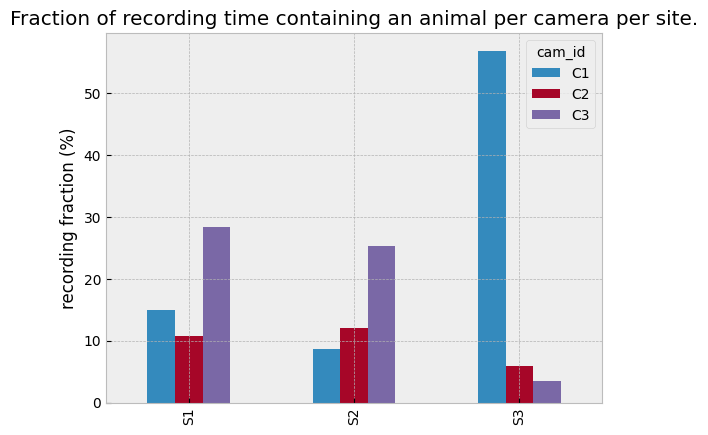
\includegraphics[width=\linewidth]{figs/raw/frac_animal.png}
      \scriptsize MegaDetector estimate per camera
    \end{column}
    \begin{column}{0.48\linewidth}
      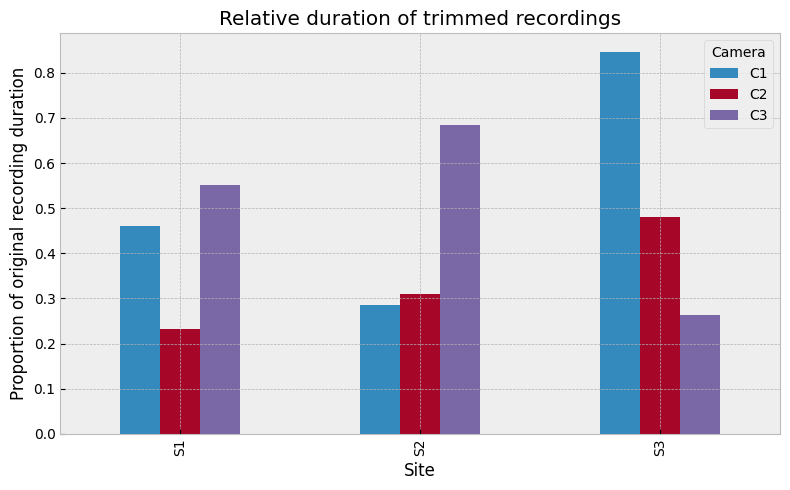
\includegraphics[width=\linewidth]{figs/trimmed/rel_dur_trimmed.png}
      \scriptsize Proportion retained after trimming
    \end{column}
  \end{columns}
  \medskip
  \alert{\textbf{80 \%} of recording time discarded, yet $\sim$11 h of real wildlife retained.}
\end{frame}

% =================================================================
% SECTION: Lessons & next steps
% =================================================================
\makesection{Takeaways}

\begin{frame}{What worked, what’s next}
  \begin{block}{Highlights}
    \begin{itemize}
      \item Full V6 integration with backward‑compatible outputs.
      \item Modular scripts \& CLI flags simplify future seasons.
      \item Pipeline feeds \textbf{MammAlps benchmarks} out of the box.
    \end{itemize}
  \end{block}
  \begin{block}{Open issues}
    \begin{itemize}
      \item Automate quality checks (false triggers, exposure quirks).
      \item Complete behavior recognition and long‑term event modules.
    \end{itemize}
  \end{block}
\end{frame}

% ----------------------------------------------------------------
\begin{frame}{Conclusion}
  \begin{itemize}
    \item 2024 run condensed \textbf{56 h $\rightarrow$ 11 h} wildlife video, 1,050 events.
    \item Upgraded detection, trimming, tracking — ready for scalable ecology.
    \item Looking forward: richer labels \& less human touch.
  \end{itemize}
  \bigskip
  \centering
  \Large\textbf{Questions?}
\end{frame}

% ----------------------------------------------------------------
\begin{frame}{Acknowledgments}
  Thanks to \textbf{Valentin Gabeff}, \textbf{Jennifer Shan}, and Prof.~\textbf{Devis Tuia}.
\end{frame}

% ----------------------------------------------------------------
\finalpagetext{Thank you for your attention!}
\makefinalpage

\end{document}
